\section{Results}


\subsection{Thrombolysis decision model}

The thrombolysis decision model predicted the probability of any patient receiving thrombolysis at any given stroke team.

Using a 80:20 train:test split, the model had an accuracy of 85\%, a balanced accuracy of 82\% (accuracy and balanced accuracy using a 50\% probability cut-off to classify a patient as a binary 'likely to receive thrombolysis' or not), and a receiver operating characteristic area under curve of 0.92 (the confusion matrix is shown in the supplementary material).

\subsection{Stroke outcome machine learning model}

Using a 80:20 train:test split, the model had a receiver operating characteristic area under curve of 0.80 (the confusion matrix is shown in the supplementary material).

\subsubsection{Prototype patients}

Prototype patients revealed variation in likely decisions between stroke teams (figure \ref{fig:thrombolysis_rates_prototype_patients}). While almost all stroke teams would give thrombolysis to the \textit{ideal} candidate for thrombolysis, the predicted use of thrombolysis varied more as one characteristic was changed from the \textit{ideal} candidate. In particular there was was a very wide range in likelihood of a patient with a mild stroke (NIHSS 3) receiving thrombolysis. Mild stroke (NIHSS < 5) represents a large proportion of admissions (54\% of all emergency stroke admissions, and 38\% of ischaemic stroke patients arriving by ambulance within 4 hours of known stroke onset). Combinations of \textit{non-ideal} patient characteristics reduced predicted use of thrombolysis further (again with significant variation between stroke teams), especially when on of the non-ideal characteristics was a mild stroke.

\begin{figure}
    \centering
    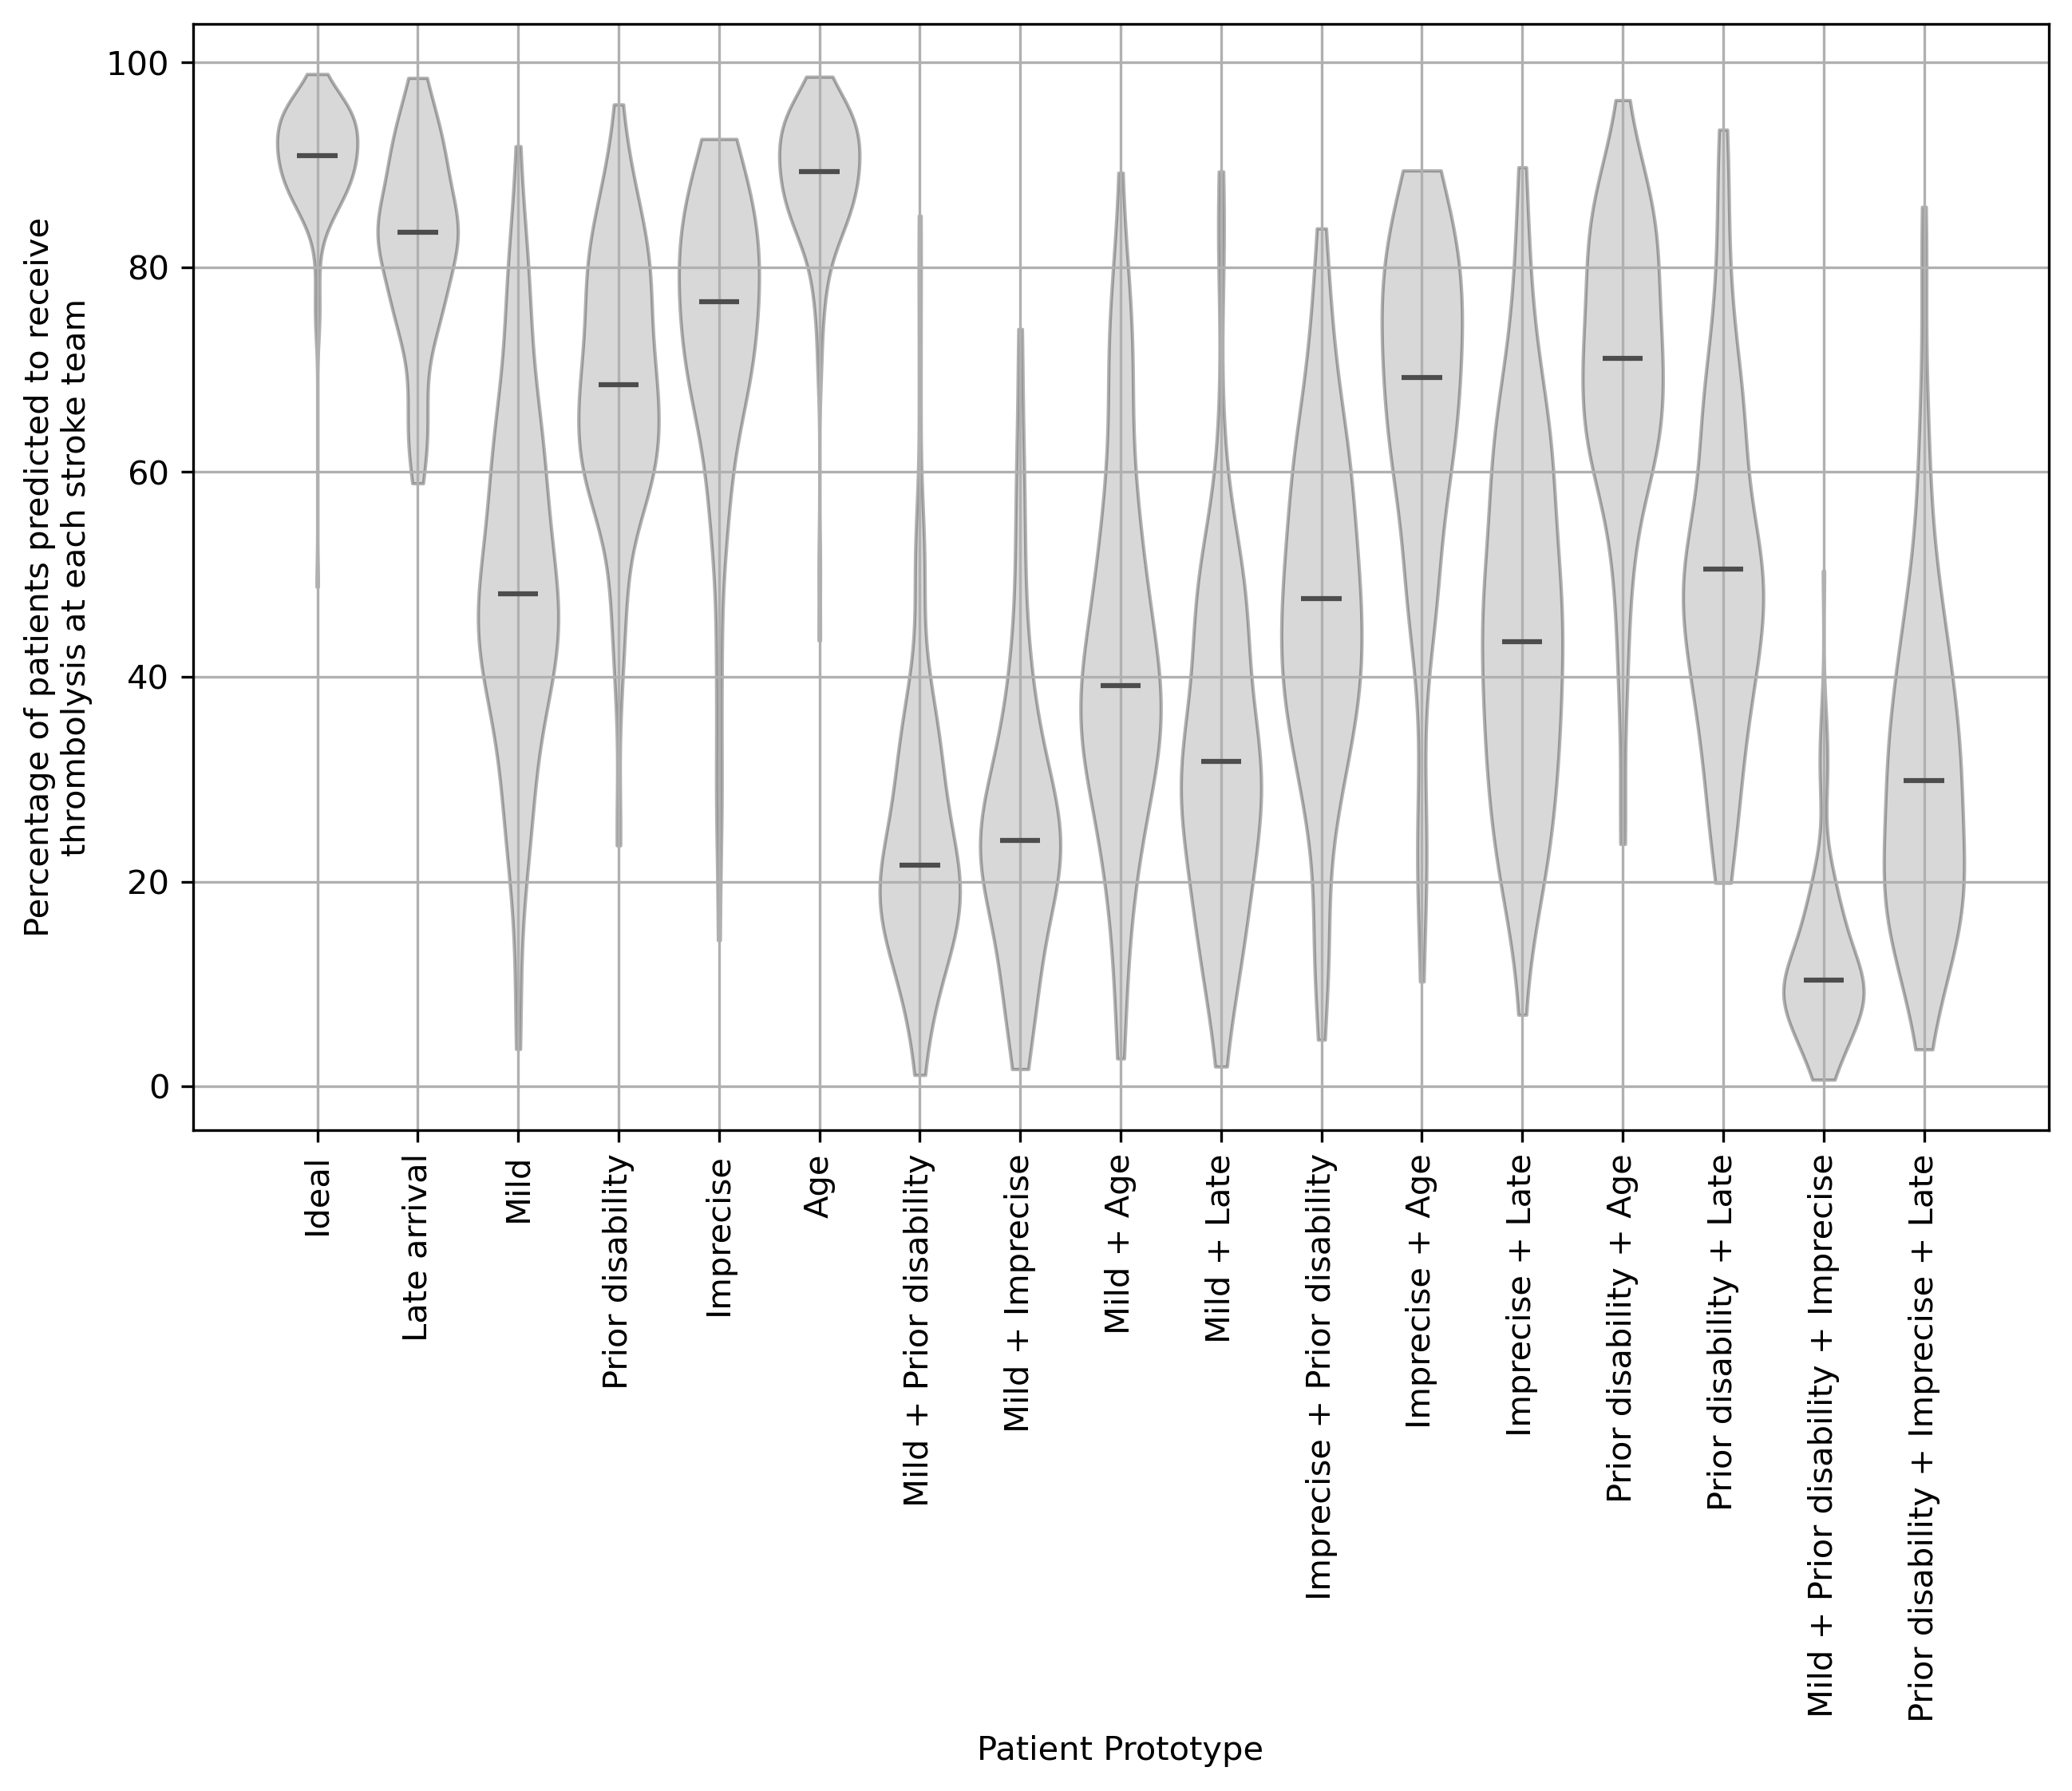
\includegraphics[width=0.75\linewidth]{images/prototype_patients_all_teams}
    \caption{Violin plots showing the variation in predicted thrombolysis rates for 17 patient prototypes across stroke teams. \textit{Ideal}: Onset-to-arrival = 90 minutes; arrival-to-scan = 15 minutes; onset-to-thrombolysis = 120 minutes; stroke severity (NIHSS) = 15; pre-stroke disability (mRS) = 0; age = 72.5; Precisely known onset; onset not during sleep; stroke type = Infarction; patient has no atrial fibrillation and is not receiving anticoagulants for atrial fibrillation; \textit{Late arrival}: as \textit{ideal} but onset-to-arrival = 225 minutes and onset-to-thrombolysis = 255 minutes \textit{Mild}: As \textit{ideal} but stroke severity = 3; \textit{Prior disability}: as \textit{ideal} but pre-stroke disability = 3; \textit{Imprecise}: as \textit{ideal} but stroke onset time estimated; \textit{Age}: as \textit{ideal} but age = 87.5.}
    \label{fig:thrombolysis_rates_prototype_patients}
\end{figure}

Figure \ref{fig:example_patient_outcome} shows an example of outcome prediction for an \textit{ideal} candidate for thrombolysis. Expected benefit from thrombolysis may be calculated as the change in the proportion of \textit{good outcomes} (e.g. mRS 0-2), the proportion of \textit{bad outcomes} (e.g. mRS 5-6), or the shift in the central point of the outcome distribution (by weighting each mRS level by the probability of being discharged with that level of disability).

\begin{figure}
    \centering
    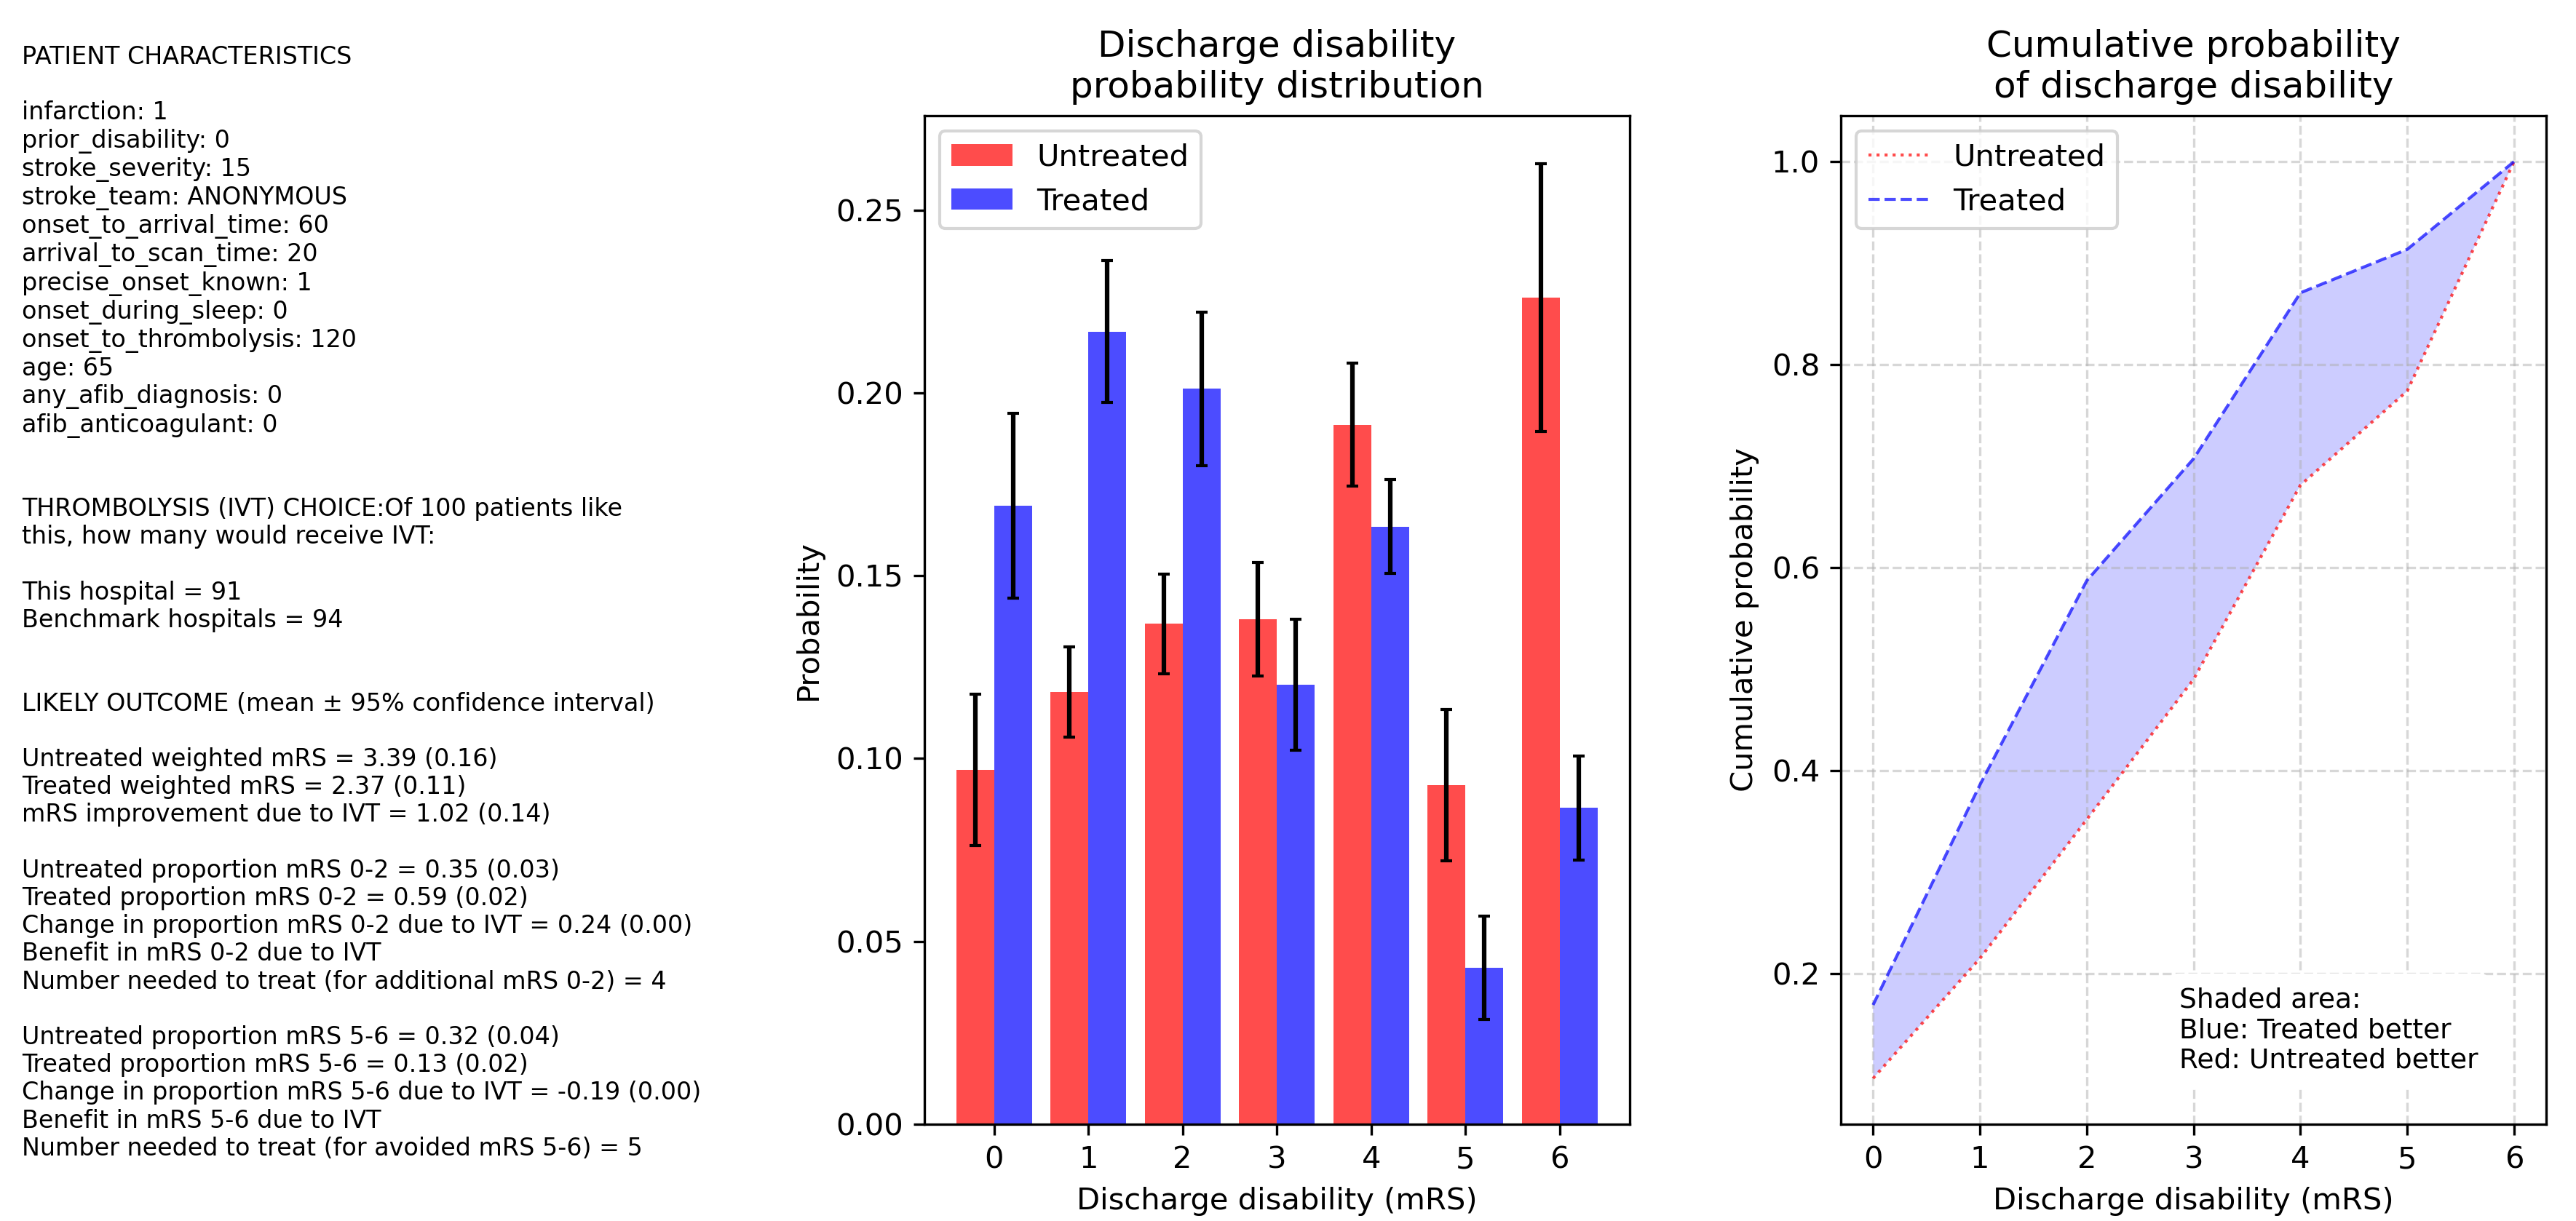
\includegraphics[width=1.0\linewidth]{images/prototype_patient_ideal}
    \caption{Enter Caption}
    \label{fig:example_patient_outcome}
\end{figure}




\subsubsection{Benchmark stroke teams and benchmark decisions}


Actual use of thrombolysis (35.1\% of 4 hour ischaemic stroke arrivals treated)
(43.2\% of 4 hour ischaemic stroke arrivals treated)








\begin{minipage}{1\textwidth}
\small
\begin{longtable}{p{5.2cm} | p{1.6cm} p{1.6cm} p{1.5cm} | p{1.6cm} p{1.6cm} p{1.5cm}}
\caption{Predicted outcomes for patient prototypes. \textit{Ideal}: Onset-to-arrival = 90 minutes; arrival-to-scan = 15 minutes; onset-to-thrombolysis = 120 minutes; stroke severity (NIHSS) = 15; pre-stroke disability (mRS) = 0; age = 72.5; Precisely known onset; onset not during sleep; stroke type = Infarction; patient has no atrial fibrillation and is not receiving anticoagulants for atrial fibrillation. \textit{Late arrival}: as \textit{ideal} but onset-to-arrival = 225 minutes and onset-to-thrombolysis = 255 minutes. \textit{Mild}; As \textit{ideal} but stroke severity = 3; \textit{Prior disability}: as \textit{ideal} but pre-stroke disability = 3; \textit{Imprecise}: as \textit{ideal} but stroke onset time estimated. \textit{Age}: as \textit{ideal} but age = 87.5. Results show probability-weighted disability at discharge, and the proportion of patients predicted to have a very poor outcome (mRS 5-6).}\\
\toprule
\endhead
Patient prototype & Untreated probability-weighted mRS & Treated probability-weighted mRS & Improve-ment & Untreated proportion mRS 5-6 & Treated proportion mRS 5-6 & Improve-ment\\
\midrule
Ideal & 3.39 & 2.37 & 1.02 & 0.32 & 0.13 & 0.19\\
Late & 3.39 & 2.73 & 0.66 & 0.32 & 0.18 & 0.14\\
Mild & 1.15 & 0.91 & 0.23 & 0.01 & 0.01 & 0.00\\
Prior disability & 4.22 & 3.61 & 0.61 & 0.41 & 0.23 & 0.19\\
Imprecise & 3.49 & 2.39 & 1.10 & 0.33 & 0.13 & 0.20\\
Age & 4.22 & 3.51 & 0.71 & 0.50 & 0.35 & 0.16\\
Mild + Prior disability & 2.92 & 2.60 & 0.32 & 0.04 & 0.04 & 0.00\\
Mild + Imprecise & 1.28 & 1.01 & 0.26 & 0.02 & 0.01 & 0.00\\
Mild + Age & 1.84 & 1.63 & 0.22 & 0.04 & 0.03 & 0.01\\
Mild + Late & 1.15 & 0.77 & 0.39 & 0.01 & 0.00 & 0.00\\
Imprecise + Prior disability & 4.33 & 3.67 & 0.66 & 0.44 & 0.24 & 0.20\\
Imprecise + Age & 4.31 & 3.57 & 0.74 & 0.53 & 0.36 & 0.17\\
Imprecise + Late & 3.49 & 2.75 & 0.74 & 0.33 & 0.17 & 0.17\\
Prior disability + Age & 4.62 & 4.35 & 0.27 & 0.53 & 0.44 & 0.08\\
Prior disability + Late & 4.22 & 3.70 & 0.52 & 0.41 & 0.27 & 0.14\\
Mild + Prior disability + Imprecise & 4.22 & 3.70 & 0.52 & 0.41 & 0.27 & 0.14\\
\bottomrule
\label{tab:prototype_outcomes}
\end{longtable}
\normalsize
\end{minipage}



\begin{figure}
    \centering
    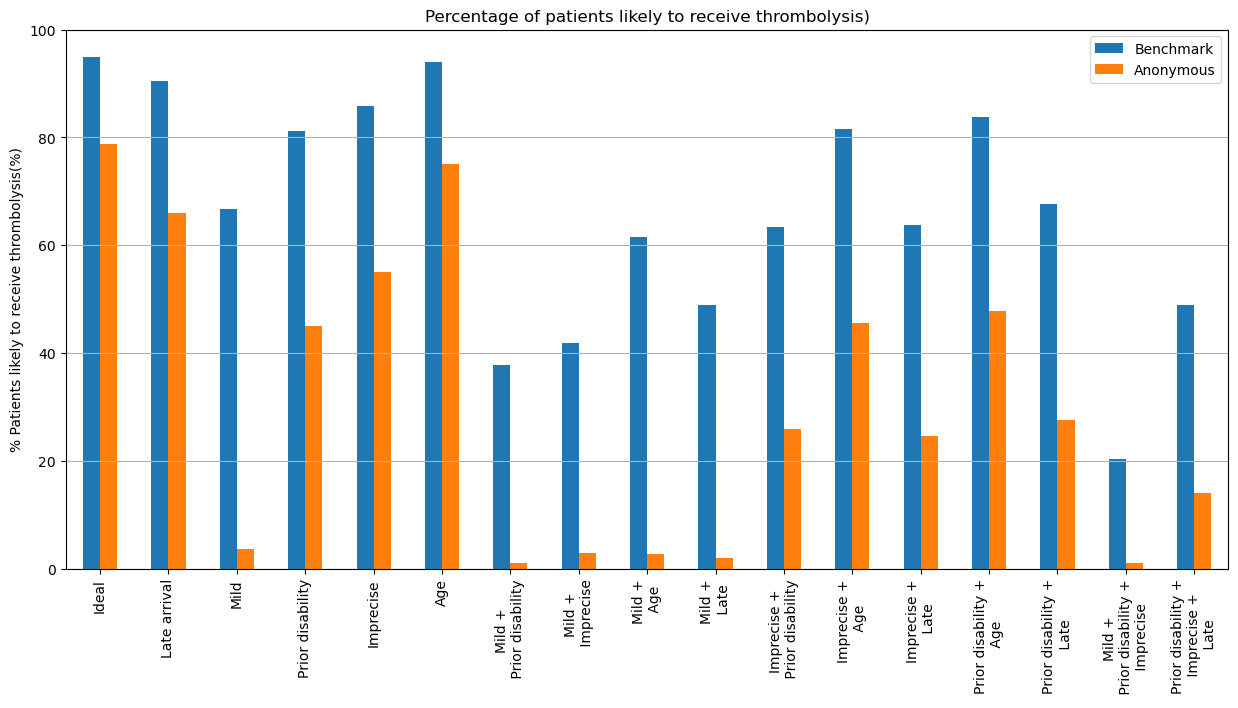
\includegraphics[width=1\linewidth]{images/prototype_patients_team_x.png}
    \caption{Enter Caption}
    \label{fig:thrombolysis_rates_prototype_patients_team_x}
\end{figure}

\subsection{Lifetime economic model}




\begin{table}
\small
\caption{Health economic analysis: Analysis for  populations based on predicted benefit (or dis-benefit) of thrombolysis. The analysis compares the populations currently treated, or the population that would be treated using \textit{benchmark} decisions (the majority vote of the predicted choice of the the 25 stroke teams most likely to use thrombolysis). Results are shown for (a) the treated populations, and (b) adjusted for 1,000 emergency stroke admissions }
\label{tab:main}

\begin{subtable}{1\textwidth}
\centering
\caption{}
\begin{tabular}{p{2.0cm} p{1.4cm} p{1.3cm} p{1.3cm} p{1.5cm} p{1.3cm} p{1.4cm} p{1.3cm} p{1.3cm}}
\toprule
Population & Group & Death & Survival (median years) & Care years (median) & QALYs & \raggedright Discounted cost per patient & Proportion mRS 0-2 & Proportion mRS 5-6\tabularnewline
\midrule
Actual & Untreated & 17.1\% & 7.60 & 0.28 & 5.020 & £20,370 & 47.1\% & 23.9\%\tabularnewline
& Treated & 14.2\% & 7.91 & 0.25 & 5.258 & £19,806 & 53.9\% & 19.3\%\tabularnewline
& Difference & -2.9\% & 0.31 & -0.03 & 0.238 & -£565 & 6.8\% & -4.7\%\tabularnewline
\midrule
Benchmark & Untreated & 17.4\% & 7.63 & 0.28 & 5.036 & £20,388 & 46.5\% & 24.1\%\tabularnewline
& Treated & 14.4\% & 7.93 & 0.25 & 5.269 & £19,784 & 53.4\% & 19.4\%\tabularnewline
& Difference & -3.0\% & 0.30 & -0.03 & 0.234 & -£603 & 6.9\% & -4.8\%\tabularnewline
\bottomrule
\end{tabular}
\end{subtable}%

\vspace{3mm}

\begin{subtable}{1\textwidth}
\centering
\caption{Analysis for 1,000 emergency stroke admissions (all stroke types)}
\begin{tabular}{p{1.9cm} p{1.9cm} p{1.9cm} p{1.9cm} p{1.9cm} p{1.9cm} p{2.2cm}}
\toprule
Population & Proportion treated & QALYs added & Healthcare costs saved & \raggedright Thrombolysis cost (£450 per patient) & \raggedright Cost per QALY added & \raggedright Net cost of thrombolysis\tabularnewline
\midrule
Actual & 11.0\% & 26.3 & £62,294 & £49,658 & £1,890 & -£12,637\tabularnewline
Benchmark & 13.6\% & 31.7 & £81,914 & £61,117 & £1,927 & -£20,797\tabularnewline
\bottomrule
\end{tabular}
\end{subtable}
\label{tab:health_econ}
\end{table}

\normalsize

\subsection{Pathway model}

\begin{figure}
    \centering
    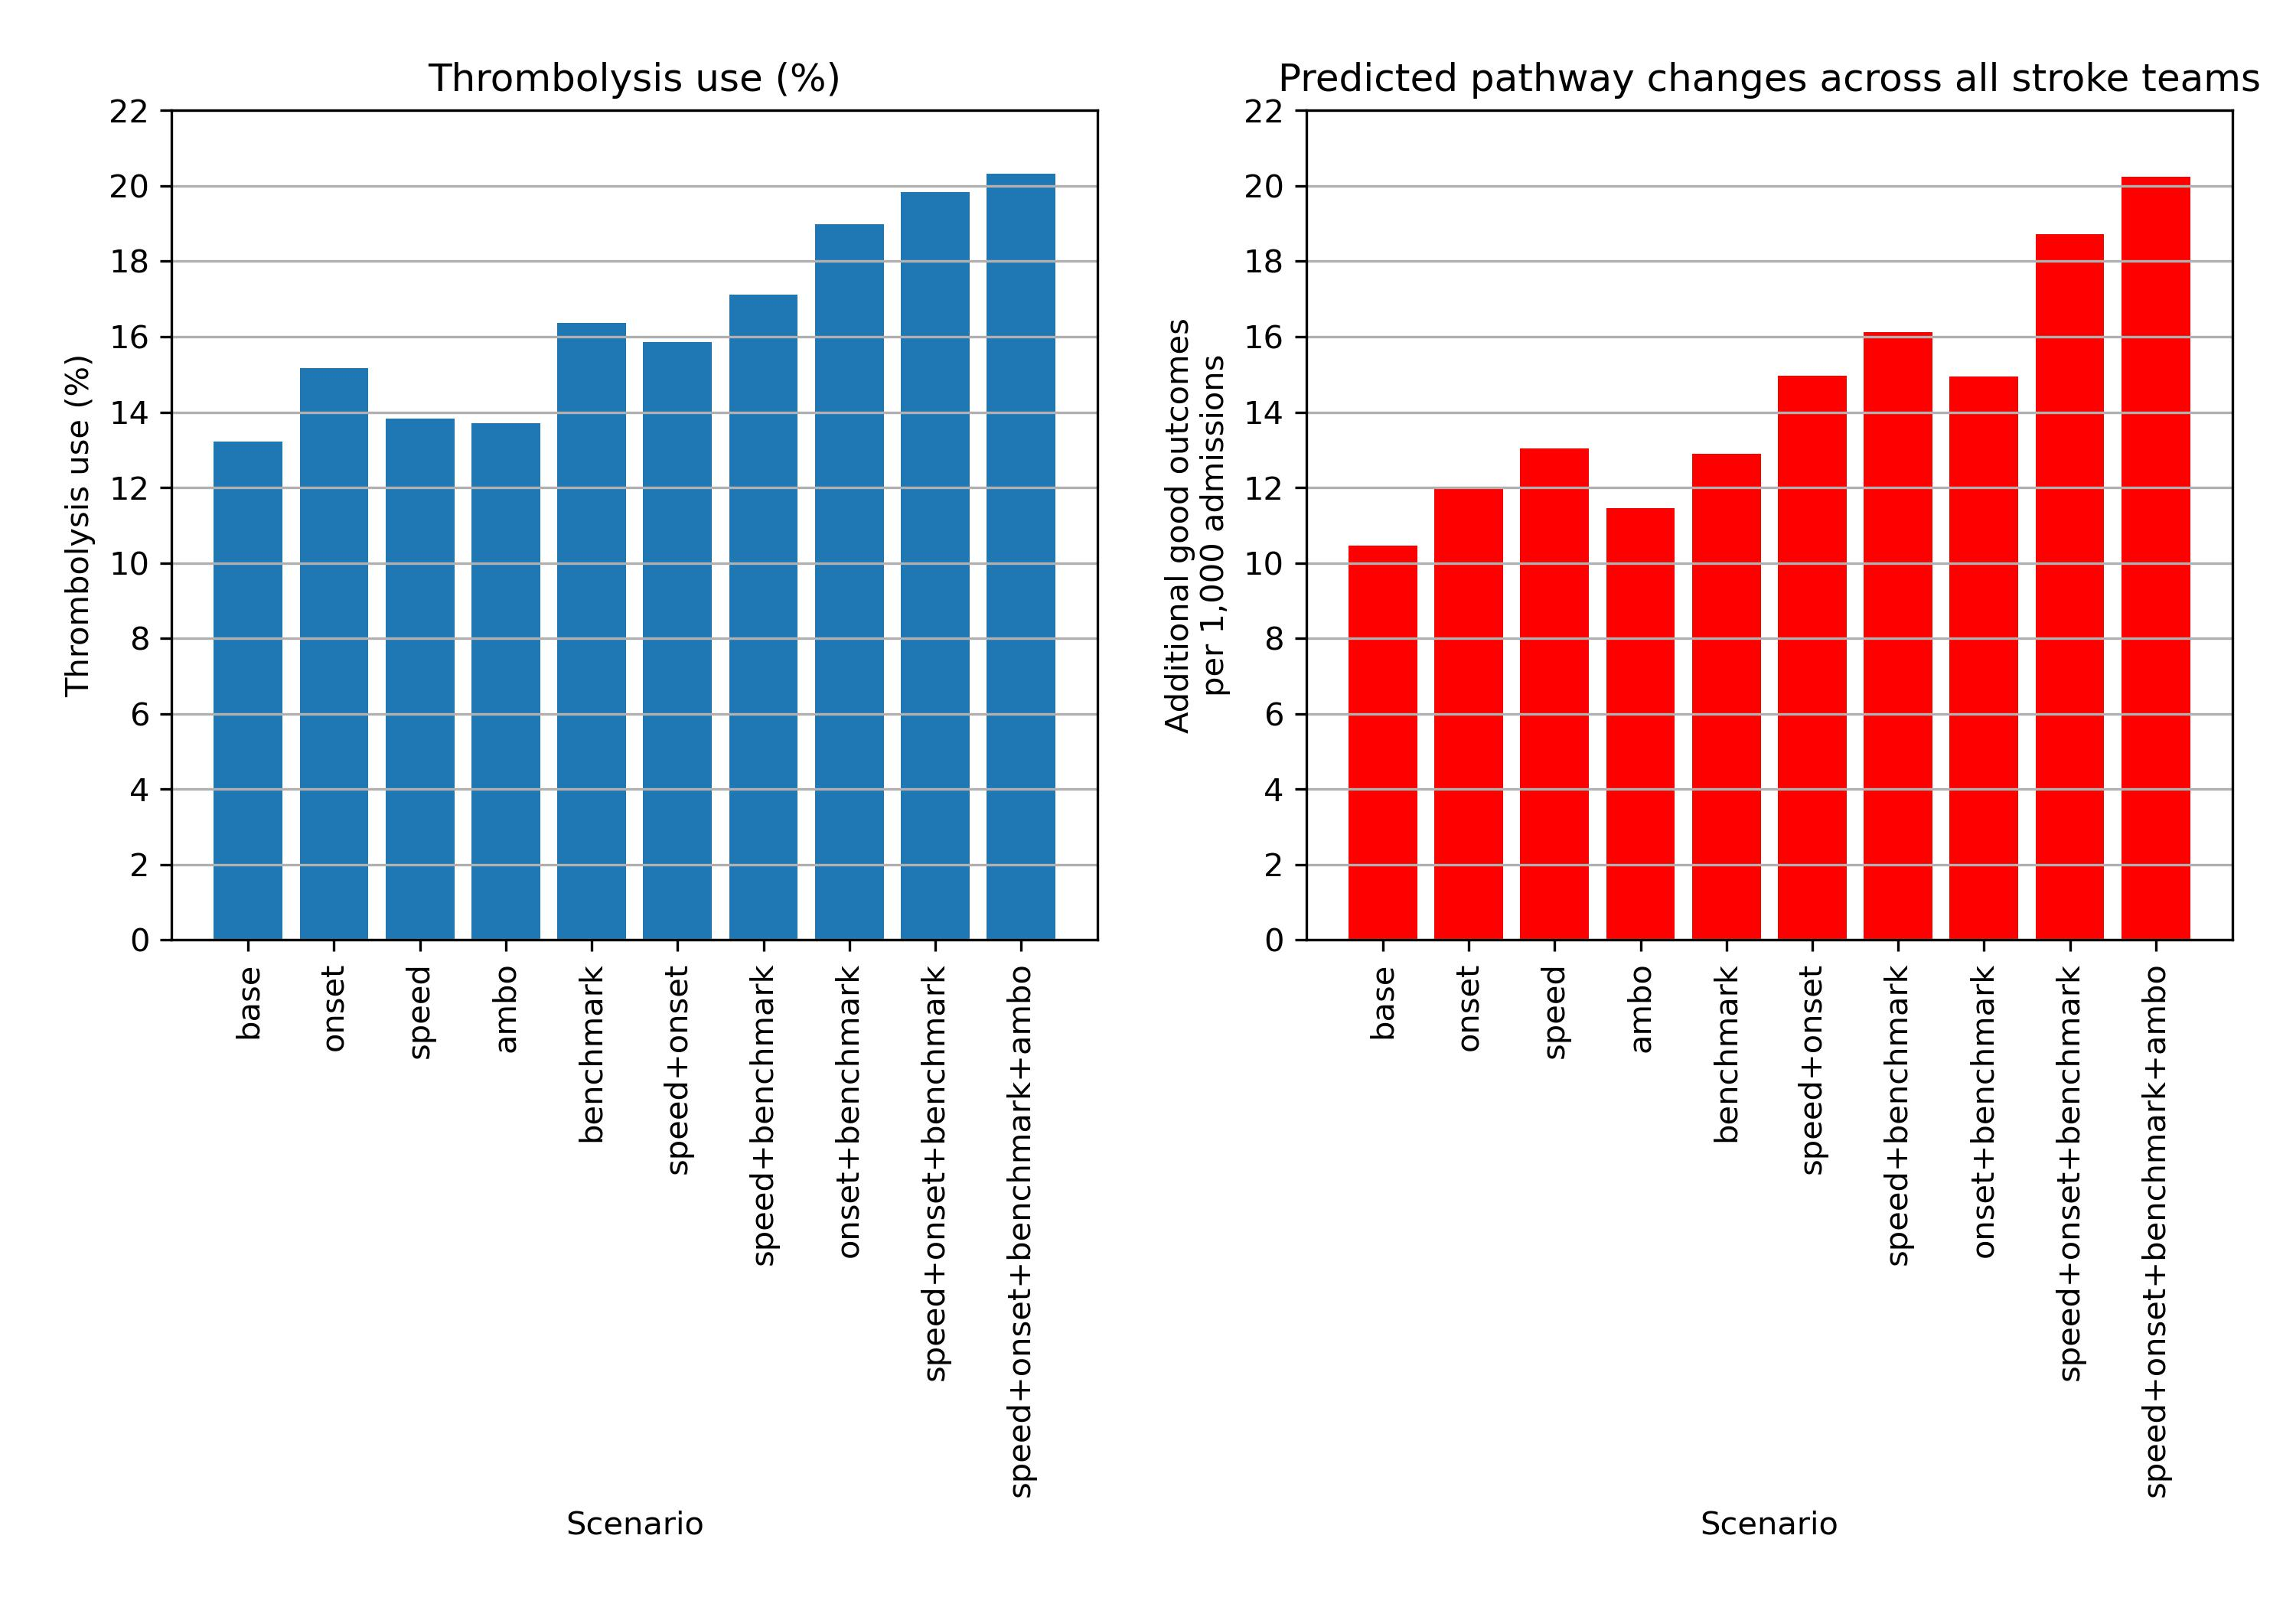
\includegraphics[width=0.75\linewidth]{images/sim_results_summary}
    \caption{Enter Caption}
    \label{fig:sim_results_summary}
\end{figure}

\begin{figure}
    \centering
    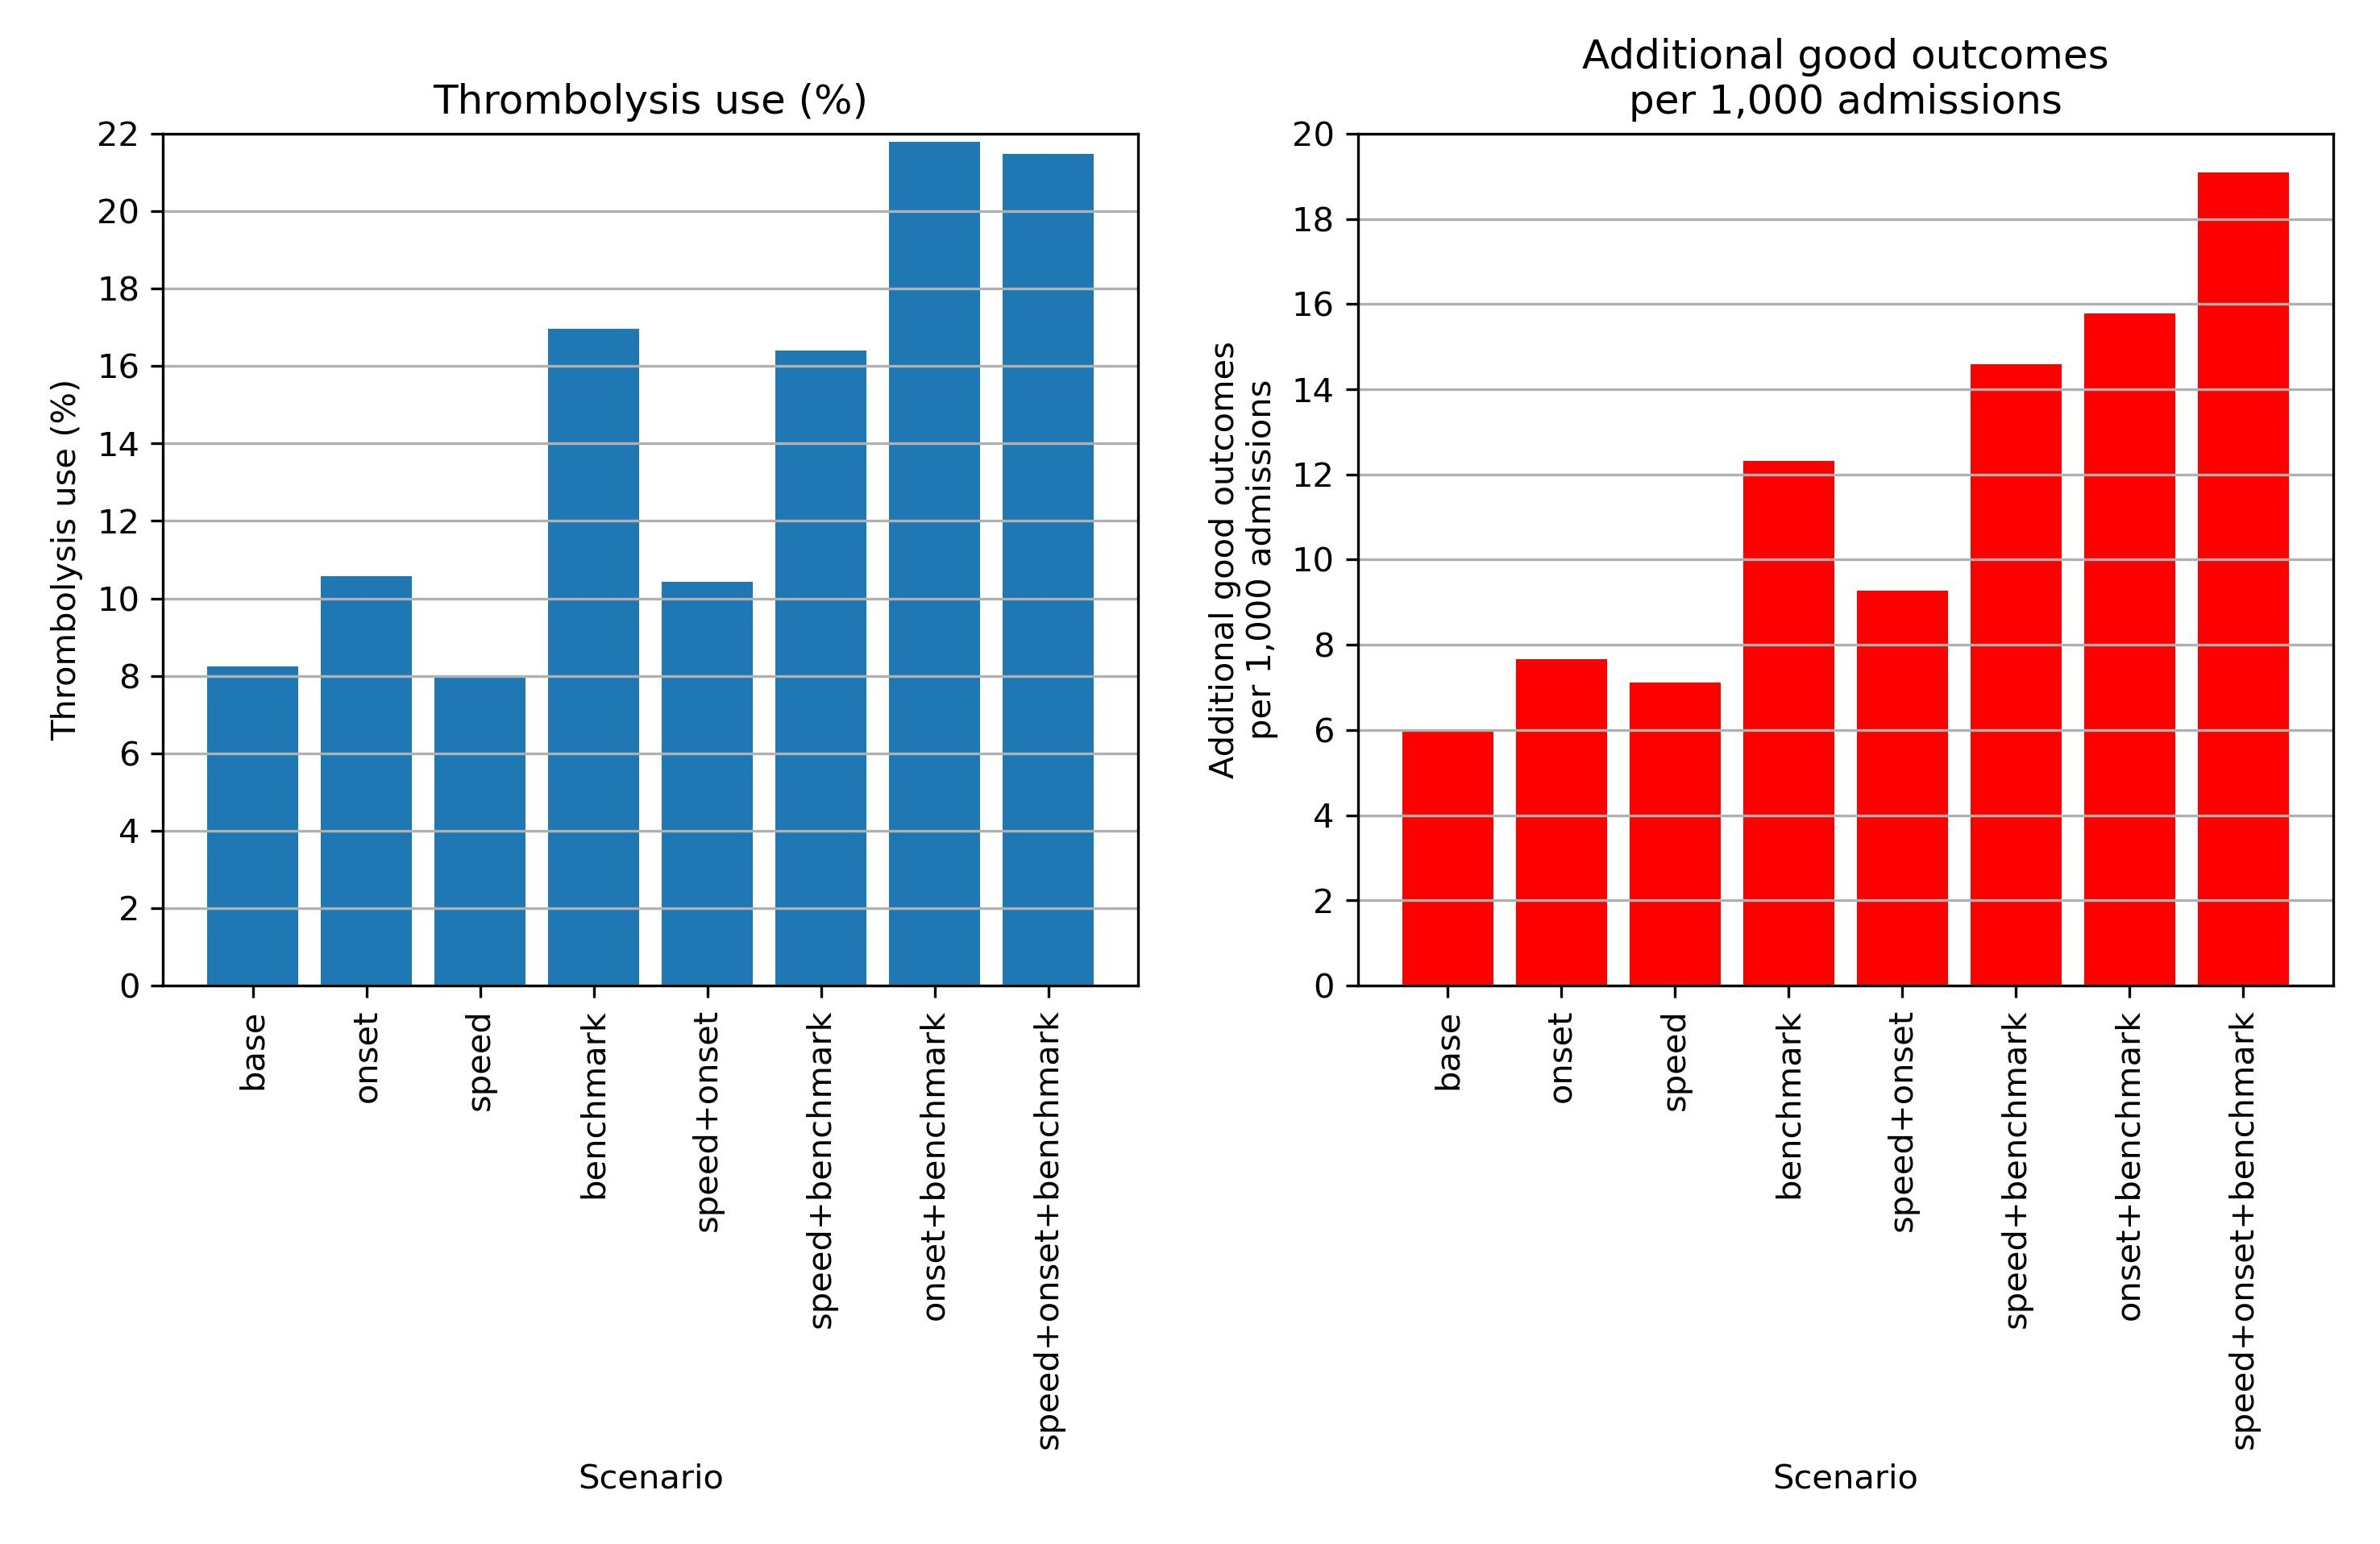
\includegraphics[width=0.75\linewidth]{images/sim_results_team_x}
    \caption{Enter Caption}
    \label{fig:sim_results_team_x}
\end{figure}








